%% For double-blind review submission, w/o CCS and ACM Reference (max submission space)
\documentclass[sigplan,10pt,review,anonymous]{acmart}
\settopmatter{printfolios=true,printccs=false,printacmref=false}
%% For final camera-ready submission, w/ required CCS and ACM Reference
%\documentclass[acmsmall]{acmart}\settopmatter{}

%\usepackage{amssymb}
\usepackage{amsmath}
\usepackage{amsfonts}
\usepackage{caption}
\usepackage{subcaption}
\usepackage{xspace}
\usepackage{mathtools}
\usepackage{mathpartir}
\usepackage{ifpdf}
\usepackage{graphicx}
%\usepackage[usenames,dvipsnames]{color}
\usepackage{stmaryrd}
%\usepackage[numbers]{natbib}
\usepackage{amsthm}
\usepackage{listings}          % format code
\usepackage{wrapfig}
\usepackage{textcomp}
\usepackage{tabularx}
\usepackage{color}
\usepackage{url}
\usepackage{tikz}
\usepackage{multirow,array}
\usepackage[utf8]{inputenc}
\usepackage[T1]{fontenc}
\usepackage{microtype}

% Math mode
%-----------
\newenvironment{nop}{}{}
\newenvironment{smathpar}{
\begin{nop}\small\begin{mathpar}}{
\end{mathpar}\end{nop}\ignorespacesafterend}
\newcounter{hypothesis}
\newenvironment{hypothesis}{\refstepcounter{hypothesis}}{}

% Theorem
%--------

\theoremstyle{plain}
\newtheorem{axiom}{Axiom}[section]
\newtheorem{theorem}{Theorem}[section]
\newtheorem{lemma}[theorem]{Lemma}
\newtheorem{proposition}[theorem]{Proposition}
\newtheorem{corollary}[theorem]{Corollary}
\theoremstyle{definition}
\newtheorem{definition}[theorem]{Definition}

\newenvironment{example}[1][Example]{\begin{trivlist}
\item[\hskip \labelsep {\bfseries #1}]}{\end{trivlist}}
\newenvironment{remark}[1][Remark]{\begin{trivlist}
\item[\hskip \labelsep {\bfseries #1}]}{\end{trivlist}}

% Decorations
%-----------
\newenvironment{decoration}
  {\color{blue}\begin{array}{l}}
  {\end{array}}

% New colors
%------------
\definecolor{Bittersweet}{rgb}{1.0, 0.44, 0.37}
\definecolor{MidnightBlue}{rgb}{0.0, 0.2, 0.4}
\definecolor{BrightBlue}{rgb}{0.0, 0.2, 0.7}

% Listings
%----------
\newcommand{\lstml}{
\lstset{ %
language=ML, % choose the language of the code
basicstyle=\footnotesize\ttfamily,       % the size of the fonts that are used for the code
keywordstyle=\color{Bittersweet},
% numbers=left,                   % where to put the line-numbers
numberstyle=\tiny,      % the size of the fonts that are used for the line-numbers
stepnumber=1,                   % the step between two line-numbers. If it is 1 each line will be numbered
numbersep=5pt,                  % how far the line-numbers are from the code
showspaces=false,               % show spaces adding particular underscores
showstringspaces=false,         % underline spaces within strings
showtabs=false,                 % show tabs within strings adding particular underscores
% frame=single,                   % adds a frame around the code
tabsize=2,                      % sets default tabsize to 2 spaces
captionpos=b,                   % sets the caption-position to bottom
breaklines=true,                % sets automatic line breaking
breakatwhitespace=false,        % sets if automatic breaks should only happen at whitespace
commentstyle=\itshape\color{BrightBlue},
%escapeinside={\%*}{*)},         % if you want to add a comment within your code
mathescape=true,
morekeywords={oper, txn, invariant, module, begin, match, when, @@deriving, not, : , txn_do, do, SQL/\\}
}}
\lstnewenvironment{ocaml}
    { % \centering
			\lstml
      \lstset{}%
      \csname lst@setfirstlabel\endcsname}
    { %\centering
      \csname lst@savefirstlabel\endcsname}
\newcommand{\ocamlinline}[1]{\lstinline[language=ML,
                                        basicstyle=\footnotesize\ttfamily, 
                                        keywordstyle=\color{Bittersweet},
                                        mathescape=true]!#1!}

% SQL Trace 
% ----------
\newcommand{\lstsql}{
\lstset{ %
  language=SQL, % choose the language of the code
  basicstyle=\footnotesize\ttfamily,       % the size of the fonts that are used for the code
  keywordstyle=\color{MidnightBlue},
  % numbers=left,                   % where to put the line-numbers
  numberstyle=\tiny,      % the size of the fonts that are used for the line-numbers
  stepnumber=1,                   % the step between two line-numbers. If it is 1 each line will be numbered
  numbersep=5pt,                  % how far the line-numbers are from the code
  showspaces=false,               % show spaces adding particular underscores
  showstringspaces=false,         % underline spaces within strings
  showtabs=false,                 % show tabs within strings adding particular underscores
  % frame=single,                   % adds a frame around the code
  tabsize=2,                      % sets default tabsize to 2 spaces
  captionpos=b,                   % sets the caption-position to bottom
  breaklines=true,                % sets automatic line breaking
  breakatwhitespace=false,        % sets if automatic breaks should only happen at whitespace
  commentstyle=\itshape\color{BrightBlue},
  %escapeinside={\%*}{*)},         % if you want to add a comment within your code
  mathescape=true,
  morekeywords={BEGIN, COMMIT, ROLLBACK}
}}
\lstnewenvironment{sqltrace}
    { % \centering
			\lstsql
      \lstset{}%
      \csname lst@setfirstlabel\endcsname}
    { %\centering
      \csname lst@savefirstlabel\endcsname}

\newcommand{\sql}[1]{\lstinline[language=SQL,
                                basicstyle=\footnotesize\ttfamily, 
                                keywordstyle=\color{BrightBlue},
                                breaklines=true,
                                breakatwhitespace=false,
                                mathescape=true,
                                morekeywords={BEGIN, COMMIT, ROLLBACK}]!#1!}


% Formatting
%---------
\newcommand{\C}[1]{\code{#1}}
\newcommand{\tuplee}[1]{\langle #1 \rangle}
\newcommand*{\rom}[1]{\expandafter\romannumeral #1}

% Formatting commands
% -------------------
\newcommand{\code}[1]{{\tt #1}}
\newcommand{\spc}[0]{\quad}
\newcommand{\ALT}{~\mid~}
\newcommand{\rel}[1]{{R}_{\mathit{#1}}}
\newcommand{\conj}{~\wedge~}
\newcommand{\disj}{~\vee~}
\newcommand{\rulelabel}[1]{\textrm{\sc {#1}}}
\newcommand{\ilrulelabel}[1]{{\sc #1}}
\newcommand{\RULE}[2]{\frac{\begin{array}{c}#1\end{array}}
                           {\begin{array}{c}#2\end{array}}}
\newcommand{\txnimp}{\mbox{${\cal T}$}}
\newcommand{\ssnimp}{{\sc SsnImp}\xspace}
%\newcommand{\coloneqq}{::=}
\newcommand{\qqquad}{\quad\quad}
\newcommand{\cskip}{\C{SKIP}}
\newcommand{\ctxn}[2]{\C{TXN}\langle #1 \rangle\{#2\}}
\newcommand{\csess}[2]{\C{ssn}\langle #1 \rangle \{#2\}}
\newcommand{\catomic}[1]{\C{ATOMIC}\{#1\}}
\newcommand{\stepsto}{\longrightarrow}
\newcommand{\stepssto}[1]{\longrightarrow^{#1}_{R}}
\newcommand{\xstepsto}[1]{\longrightarrow_{#1}}
\newcommand{\xstepssto}[2]{\longrightarrow^{#1}_{#2}}
\newcommand{\tstepsto}{\longrightarrow}
\newcommand{\redsto}{\hookrightarrow}
\newcommand{\xtstepsto}[1]{\hookrightarrow_{#1}}
\newcommand{\rtstepsto}{\hookrightarrow_R}
\newcommand{\rtstepssto}[1]{\hookrightarrow^{#1}_R}
\newcommand{\xtstepssto}[2]{\hookrightarrow^{#1}_{#2}}
\newcommand{\hoare}[3]{\{#1\}\,#2\,\{#3\}}
\newcommand{\defeq}[0]{\overset { \mathit{def} }{ = } }
\newcommand{\rg}[3]{\{#1\}\,#2\,\{#3\}}
%\newcommand{\defeq}[0]{ \triangleq }
\newcommand{\op}{\textsf{op}}
\newcommand{\E}{\mathcal{E}}
\newcommand{\I}{\mathbb{I}}
\newcommand{\F}{{\sf F}}
\newcommand{\G}{{\sf G}}
\newcommand{\D}{\mathcal{D}}
\newcommand{\T}{\mathcal{T}}
\renewcommand{\P}{\mathcal{P}}
\newcommand{\Lfull}{L}
\newcommand{\Lnoloop}{L_{\diamond}}
\newcommand{\Lnoif}{L_{\downarrow}}
\newcommand{\visZ}{\textsf{vis}}
\newcommand{\soZ}{\textsf{so}}
\newcommand{\hbZ}{\textsf{hb}}
\newcommand{\sameobj}[2]{\textsf{sameobj}(#1,#2)}
\newcommand{\sameobjZ}{\textsf{sameobj}}
\newcommand{\visar}{\xrightarrow{\visZ}}
\newcommand{\hboar}{\xrightarrow{\textsf{hb}}}
\newcommand{\soar}{\xrightarrow{\soZ}}
\newcommand{\visoar}{\xrightarrow{\visZ \,\cup\, \soZ}}
\newcommand{\invisar}{\xrightarrow{\textsf{invis}}}
\newcommand{\etaar}{\xrightarrow{\eta}}
\newcommand{\wrstoar}{\xrightarrow{\textsf{wrsto}}}
\newcommand{\rdsfmar}{\xrightarrow{\textsf{rdsfm}}}
\newcommand{\usesar}{\xrightarrow{\textsf{uses}}}
\newcommand{\isReadf}{\textsf{isRD}}
\newcommand{\isWritef}{\textsf{isWR}}
\newcommand{\oper}{\textsf{oper}}
\newcommand{\committed}{\textsf{com}}
\newcommand{\txn}{\textsf{txn}}
\newcommand{\ssn}{\textsf{ssn}}
\newcommand{\id}{\textsf{id}}
\newcommand{\kind}{\textsf{oper}}
\newcommand{\obj}{\textsf{obj}}
\newcommand{\rval}{\textsf{rval}}
\newcommand{\visible}{\textsf{visible}}
\newcommand{\maxId}{\textsf{maxId}}
\newcommand{\aeval}{\textsf{aeval}}
\newcommand{\underE}[1]{\E \Vdash #1}
\newcommand{\underIT}[1]{\;\I,\C{Txn}_i \vdash #1\;}
\newcommand{\underI}[1]{\;\I \vdash #1\;}
\newcommand{\underT}[1]{\;\C{Txn}_i \vdash #1\;}
\newcommand{\stable}{\mathtt{stable}}
\newcommand{\iso}[1]{\emph{#1}}
\newcommand{\writef}{\textsf{Write}}
\newcommand{\readf}{\textsf{Read}}
\newcommand{\commitf}{\textsf{Commit}}
\newcommand{\eg}{\emph{e.g.,}}
\newcommand{\GK}[1]{\textcolor{red}{#1}}
\newcommand{\SJ}[1]{\textcolor{red}{SJ: #1}}
\newcommand{\valid}{\textsf{valid}}

\newcommand{\B}[1]{\small\bf #1}
\newcommand{\txnbox}[1]{\lbrack #1 \rbrack}
\newcommand{\Prop}{\mathbb{P}}
\newcommand{\Pow}[1]{\mathcal{P}\left(#1\right)}
\renewcommand{\bar}[1]{\overline{#1}}
\renewcommand{\merge}{\diamond}
\newcommand{\quark}{{\sc Quark}\xspace}
\newcommand{\hlabel}[1]{\begin{hypothesis}\label{#1}\end{hypothesis}\ref{#1}}
\newcommand{\A}{\mathcal{A}}
\newcommand{\entails}{\vDash}
\newcommand{\M}{\mathcal{M}}
\newcommand{\colondash}{~\operatorname{:-}~}
\newcommand{\cedge}{\xrightarrow{c}}
\newcommand{\fedge}{\xrightarrow{f}}
\newcommand{\medge}{\xrightarrow{m}}
\newcommand{\fmedges}{\xrightarrow{f,m}\!\!^{*}}
\newcommand{\reaches}{\rightarrow^{*}}
\newcommand{\reachable}{\leftrightarrow^{*}}

% Low-level reduction relation
\newcommand{\rightarrowdbl}{\rightarrow\mathrel{\mkern-14mu}\rightarrow}

\newcommand{\xrightarrowdbl}[2][]{%
  \xrightarrow[#1]{#2}\mathrel{\mkern-14mu}\rightarrow
}
\newcommand{\qstepsto}{\xrightarrowdbl{\spc}}



%% Journal information
%% Supplied to authors by publisher for camera-ready submission;
%% use defaults for review submission.
\acmJournal{PACMPL}
\acmVolume{1}
\acmNumber{POPL} % CONF = POPL or ICFP or OOPSLA
\acmArticle{1}
\acmYear{2022}
\acmMonth{1}
\acmDOI{} % \acmDOI{10.1145/nnnnnnn.nnnnnnn}
\startPage{1}

%% Copyright information
%% Supplied to authors (based on authors' rights management selection;
%% see authors.acm.org) by publisher for camera-ready submission;
%% use 'none' for review submission.
\setcopyright{none}
%\setcopyright{acmcopyright}
%\setcopyright{acmlicensed}
%\setcopyright{rightsretained}
%\copyrightyear{2018}           %% If different from \acmYear

%% Bibliography style
\bibliographystyle{ACM-Reference-Format}
%% Citation style
%% Note: author/year citations are required for papers published as an
%% issue of PACMPL.
\citestyle{acmauthoryear}   %% For author/year citations


%%%%%%%%%%%%%%%%%%%%%%%%%%%%%%%%%%%%%%%%%%%%%%%%%%%%%%%%%%%%%%%%%%%%%%
%% Note: Authors migrating a paper from PACMPL format to traditional
%% SIGPLAN proceedings format must update the '\documentclass' and
%% topmatter commands above; see 'acmart-sigplanproc-template.tex'.
%%%%%%%%%%%%%%%%%%%%%%%%%%%%%%%%%%%%%%%%%%%%%%%%%%%%%%%%%%%%%%%%%%%%%%


\begin{document}

%% Title information
\title[]{Runtime-Assisted Convergence in Replicated Data Types}
%% [Short Title] is optional;
                                        %% when present, will be used in
                                        %% header instead of Full Title.
%\titlenote{with title note}             %% \titlenote is optional;
                                        %% can be repeated if necessary;
                                        %% contents suppressed with 'anonymous'
%\subtitle{Subtitle}                     %% \subtitle is optional
%\subtitlenote{with subtitle note}       %% \subtitlenote is optional;
                                        %% can be repeated if necessary;
                                        %% contents suppressed with 'anonymous'


%% Author information
%% Contents and number of authors suppressed with 'anonymous'.
%% Each author should be introduced by \author, followed by
%% \authornote (optional), \orcid (optional), \affiliation, and
%% \email.
%% An author may have multiple affiliations and/or emails; repeat the
%% appropriate command.
%% Many elements are not rendered, but should be provided for metadata
%% extraction tools.

%% Author with single affiliation.
\author{First1 Last1}
\authornote{with author1 note}          %% \authornote is optional;
                                        %% can be repeated if necessary
\orcid{nnnn-nnnn-nnnn-nnnn}             %% \orcid is optional
\affiliation{
  \position{Position1}
  \department{Department1}              %% \department is recommended
  \institution{Institution1}            %% \institution is required
  \streetaddress{Street1 Address1}
  \city{City1}
  \state{State1}
  \postcode{Post-Code1}
  \country{Country1}                    %% \country is recommended
}
\email{first1.last1@inst1.edu}          %% \email is recommended

%% Author with two affiliations and emails.
\author{First2 Last2}
\authornote{with author2 note}          %% \authornote is optional;
                                        %% can be repeated if necessary
\orcid{nnnn-nnnn-nnnn-nnnn}             %% \orcid is optional
\affiliation{
  \position{Position2a}
  \department{Department2a}             %% \department is recommended
  \institution{Institution2a}           %% \institution is required
  \streetaddress{Street2a Address2a}
  \city{City2a}
  \state{State2a}
  \postcode{Post-Code2a}
  \country{Country2a}                   %% \country is recommended
}
\email{first2.last2@inst2a.com}         %% \email is recommended
\affiliation{
  \position{Position2b}
  \department{Department2b}             %% \department is recommended
  \institution{Institution2b}           %% \institution is required
  \streetaddress{Street3b Address2b}
  \city{City2b}
  \state{State2b}
  \postcode{Post-Code2b}
  \country{Country2b}                   %% \country is recommended
}
\email{first2.last2@inst2b.org}         %% \email is recommended


%% Abstract
%% Note: \begin{abstract}...\end{abstract} environment must come
%% before \maketitle command
\begin{abstract}
   Programming geo-distributed replicated systems is hard given the
   complexity of reasoning about constantly evolving states at different
   replicas. Uncoordinated updates to replicas lead to states that are
   unlikely to converge. In the absence of inter-replica coordination,
   commutativity has come to be accepted as the \emph{de facto} design
   principle to guarantee convergence. Unfortunately, designing replicated
   state updates as commutative operations is hard considering that most
   data types define operations that do not commute. Deriving a replicated
   variant of a data type often entails a creative re-engineering of its
   internal representation and algorithms so as to support commutative
   operations while retaining (close to) the original semantics. In this
   paper we propose an alternative approach to replicated data types that
   avoids such complex re-engineering. Our approach is fundamentally
   different in that it is based on the weaker notion of
   \emph{mergeability}. Unlike commutativity, mergeability only requires a
   data type to define \emph{a} merge semantics while leaving its existing
   definition intact. Notably, our approach leaves type and merge semantics
   completely unconstrained even as it guarantees eventual convergence and
   full availability in an asynchronous distributed setting. In other
   words, there is no need for the programmers to prove algebraic
   properties of their implementations in order to obtain the convergence
   and availability guarantees under a distributed execution. Such
   weakening of obligations is made possible by a novel distributed runtime
   that orchestrates distributed executions as per a structural
   well-formedness criterion, which we show is sufficient to guarantee
   convergence. We implement the runtime called \quark as a thin shim layer
   on top of an off-the-shelf distributed database, and use it to run
   mergeable replicated variants of several ordinary data types. Our
   evaluation categorically demonstrate the generality of our approach and
   the low overhead imposed by our runtime.

\end{abstract}


%% 2012 ACM Computing Classification System (CSS) concepts
%% Generate at 'http://dl.acm.org/ccs/ccs.cfm'.
\begin{CCSXML}
<ccs2012>
<concept>
<concept_id>10011007.10011006.10011008</concept_id>
<concept_desc>Software and its engineering~General programming languages</concept_desc>
<concept_significance>500</concept_significance>
</concept>
<concept>
<concept_id>10003456.10003457.10003521.10003525</concept_id>
<concept_desc>Social and professional topics~History of programming languages</concept_desc>
<concept_significance>300</concept_significance>
</concept>
</ccs2012>
\end{CCSXML}

\ccsdesc[500]{Software and its engineering~General programming languages}
\ccsdesc[300]{Social and professional topics~History of programming languages}
%% End of generated code


%% Keywords
%% comma separated list
\keywords{keyword1, keyword2, keyword3}  %% \keywords are mandatory in final camera-ready submission


%% \maketitle
%% Note: \maketitle command must come after title commands, author
%% commands, abstract environment, Computing Classification System
%% environment and commands, and keywords command.
\maketitle


\section{Introduction}
\label{sec:intro}

Large-scale web services and decentralized applications often rely on
geo-distributed state replication to meet their latency and availability
needs. An application's state is replicated asynchronously in such a
setting, meaning that operations are independently executed at each
replica, and updates are applied asynchronously at other replicas after a
possible network delay. Asynchronous execution complicates programming and
reasoning about distributed applications as it induces the possibility of
conflicting updates leading to non-convergence and application integrity
violations. Two basic approaches have been proposed to address this
problem. The first approach is to selectively strengthen the system
consistency to pre-empt the conflicting updates. The second is to redefine
the application state in terms of \emph{Replicated Data Types} (RDTs) that
are specially engineered to handle conflicting updates. Strengthening
system consistency necessarily entails inter-replica coordination,
therefore applications prefer to utilize RDTs as much as possible,
resorting to consistency strengthening only when it is necessary to maintain
application integrity. The common design principle guiding the development
of replicated data types is commutativity. The idea is that if the
replicated state is only updated by commutative operations, then updates
can be applied in any order and the replica states are still guaranteed to
converge. Indeed, there exist common usecases in web applications that can
be implemented using Commutative Replicated Data Types
(CRDTs)~\cite{crdts}. For instance, a video view counter on a streaming
application such as YouTube can be implemented as a Counter CRDT that
supports commutative increments.

In general, however, commutativity is not a common occurrence among
data types. Most common data type definitions come with at least a
pair of operations that do not commute. For instance an \C{add} and a
\C{remove} operations on a set do not commute if both are for the same
element.  Likewise two \C{insert} operations for the same position in
a list do not commute. Such non-commutative operations translate to
conflicting updates in a distributed setting, whose cumulative result
cannot be determined by the sequential specification of the data type
alone. To use a non-commutative data type in a replicated setting,
creative re-engineering of its internal representation and algorithms
is needed to turn it into a bonafide CRDT with a sensible distributed
semantics.
% In the case of set data type, that could involve changing the internal
% representation to maintain two sets -- a set containing the current
% elements and a \emph{tombstone} set that contains every element that
% has ever been deleted from the set. A \C{remove $k$} operation removes
% $k$ from the element set and adds it to the tombstone set, and an
% \C{insert $k$} operation adds $k$ to the element set only if it is not
% present in the tombstone set (i.e., only if $k$ was not previously
% deleted from the set). This results in a CRDT set called
% \emph{two-phase set} where an element once removed cannot be re-added. 
% A more complex re-engineering of the set data type could result in a set
% CRDT with a different (and arguably more useful) semantics.
% Sec.~\ref{sec:motivation} describes a \emph{remove-wins} CRDT set, which
% allows elements to be readded, but which prioritizes \C{remove}s over
% concurrent \C{insert}s. This transformation requires vector
% clocks~\cite{vectorclock} to keep track of casual ordering among
% \C{insert}s and \C{remove}s.
Indeed, most CRDTs have such carefully-crafted implementations that
rely on non-trivial technical devices to keep track of causal
dependencies and avoid or resolve conflicts. For instance, various
CRDT variants of the set abstract data type rely on \emph{vector
clocks} to identify conflicting \C{add}s and
\C{remove}s~\cite{zawirski-thesis, zhang}, Replicated Growable Array
(RGA) -- a CRDT for collaborative editing~\cite{rga}, and JSON CRDT --
a CRDT variant of the JSON storage format, both use \emph{Lamport
timestamps}~\cite{rga, json-crdt}; and TreeDoc, another CRDT for
collaborative editing, makes use of \emph{dense linear
orders}~\cite{treedoc}. Such advanced implementations makes it hard to
reason about basic correctness properties of CRDTs, such as
convergence. Indeed, formal verification of \emph{strong eventual
consistency} (i.e., eventual convergence) for few of the
aforementioned CRDTs required considerable effort on behalf of
multiple authors who are experts in the field~\cite{kleppmann2017}.
The extraordinary effort and the expertise required to build CRDTs is
a deterrent towards using type-safe abstractions with strong
guarantees in distributed applications. To overcome this deterrent,
there is a need for an alternative approach that lets developers reuse
their sequential abstractions in a distributed setting with little to
no additional overhead of reasoning about their correctness properties
such as convergence.

% hinders the widespread adoption of replicated data
% types in software development.
In this paper we propose such an alternative approach to convergent
replicated data types. The key distinguishing characteristic of our
approach is the utilization of a distributed runtime to orchestrate
\emph{well-formed} distributed executions that are guaranteed to
converge. We define well-formedness as a constraint over the
\emph{states} that arise during the execution as opposed to the
\emph{operations} that are involved in the execution. To allow for its
enforcement, we adopt a state-centric model of replication based on
version-controlled \emph{mergeable} states~\cite{mrdt} instead of an
operation-centric model based on commutative operations. Unlike
commutativity, mergeability does not require a data type definition to
be refactored to suit distributed execution. Instead, the type
definition only needs to be extended with a \C{merge} function to
reconcile concurrent versions of the type in presence of their common
ancestor version. Notably, \C{merge} function is left completely
unconstrained. Consequently, programmer can chose any merge semantics
that make sense within the context of the data type's (sequential)
semantics without risking the loss of convergence. Such strong
guarantees are made possible by the simplicity of state-based
reasoning combined with the run-time enforcement of well-formedness. 

% combined with the simplicity
% of state-based reasoning. Note that state-centric model of
% replication has also been explored in the context of CRDTs. However,
% state-based CRDTs require the replicated state to be organized as a
% lattice -- a restriction we relax in our setting. 

Note that it is easy to construct a trivial runtime that guarantees
convergence of all executions.  Such a runtime would make an extensive
use of inter-replica coordination to synchronize the execution of
every operation and thus induce a sequentially-consistent behavior.
This would however defeat the purpose of state replication as the
latency incurred for synchronized execution of an operation is
prohibitively high, and the availability of the system during the
execution is correspondingly low. It is therefore important for a
distributed runtime of RDTs to not synchronize the execution of RDT
operations. Orchestrating a well-formed convergent execution without
impacting latency and availability may seem impossible due to the CAP
theorem~\cite{cap}, but it is not the case in fact. While CAP theorem
does rule out linearizability, it does not prohibit enforcing weaker
consistency constraints on distributed executions. Our approach
exploits this observation by (\rom{1}). Identifying a novel set of
constraints on distributed executions that guarantee their
convergence, and (\rom{2}). Localizing such constraints on
(asynchronously executed) state merges such that per-operation latency
and system-wide availability remain unaffected.
Sec.~\ref{sec:concrete-sem} explains our runtime in detail.

% In fact many CRDTs,
% including the aforementioned \emph{remove-wins} set, implicitly assume
% \emph{causal consistency}, which is weaker than linearizability but is
% stronger than the default \emph{eventual consistency}. While causal
% consistency alone cannot guarantee convergence, it sufficiently
% constrains the distributed execution for the CRDT implementations to
% guarantee convergence. In this respect our approach differs in the
% sense that  

\paragraph{Contributions} The contributions of this paper are summarized
below:
\begin{itemize}
  \item We present a runtime-assisted approach to state replication
    that sufficiently constrains distributed executions so as to
    guarantee the convergence of replicated data types. This is in
    contrast to the existing models of replication, where each type is
    obligated to prove its convergence.

  \item We formalize the aforementioned constraints in the context of
    a an abstract machine (named \quark) that manifests distributed
    executions as version history graphs (similar to Git~\cite{git}).
    We prove the \emph{convergence} and \emph{progress} properties of
    the \quark abstract machine that together guarantee its soundness.
    The formalization has been mechanized in Ivy~\cite{ivy} and
    \emph{automatically} verified with help of Z3~\cite{z3}. To the
    best of our knowledge, this is the first time an SMT solver was
    used to verify the \emph{meta-theory} of a formal system.

  \item We formalize \quark distributed machine that implements the
    semantics of the \quark abstract machine in the context of an
    asynchronous distributed system. The formalization addresses
    several practical concerns of distribution and serves as a
    blueprint for an efficient implementation.

  \item We describe an implementation of \quark as a light-weight shim
    layer on top of Scylla -- an off-the-shelf distributed key-value
    store~\cite{scylla}. We evaluate the implementation on a
    collaborative-editing benchmark to demonstrate novel trade-offs
    presented by our approach.
\end{itemize}



\section{Motivation}
\label{sec:motivation}


In this section we motivate our runtime-assisted approach to
convergent RDTs with help of a set data structure.

\begin{figure}[ht]
\centering
\begin{ocaml}
module Set: sig
  type t (* Abstract type of the set*)    
  type elt (* Abstract type of set elements *)
  val add: elt -> unit (*Add an element *)
  val remove: elt -> unit (* Remove an element *)
end
\end{ocaml}
\caption{An OCaml interface to \C{Set} abstract data type}
\label{fig:ocaml-set}
\end{figure}

\begin{figure}[ht]
  \centering
  \begin{subfigure}[t]{0.55\columnwidth}
    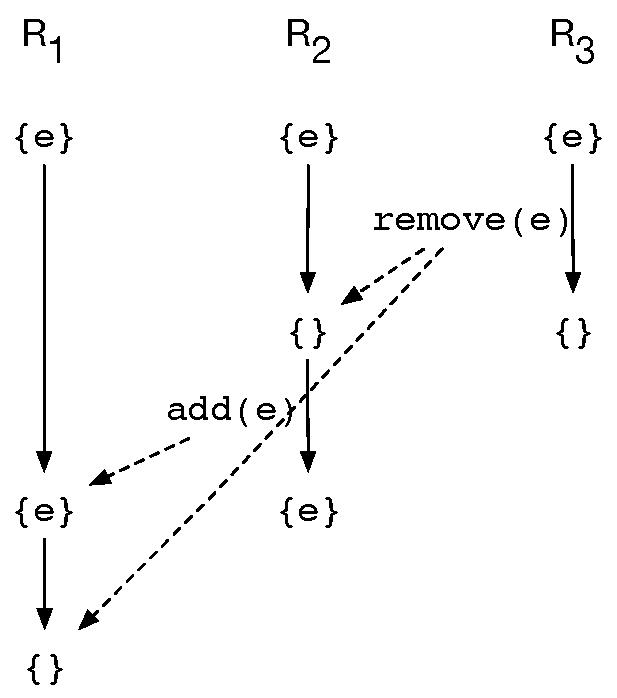
\includegraphics[scale=0.35]{Figures/crdt-execs-1}
    \caption{}
    \label{fig:crdt-execs-1}
  \end{subfigure}
  \begin{subfigure}[t]{0.44\columnwidth}
    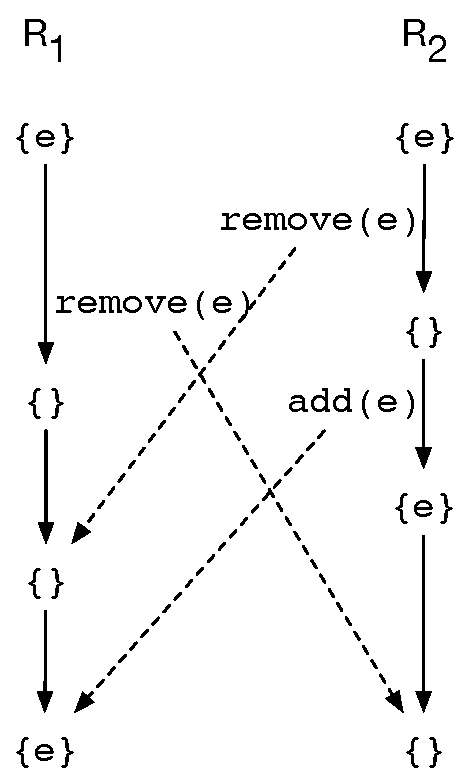
\includegraphics[scale=0.35]{Figures/crdt-execs-2}
    \caption{}
    \label{fig:crdt-execs-2}
  \end{subfigure}
\caption{Anamolous executions resulting from the Asynchronous
  replication of \C{Set}. Dashed lines denote effect propagation.}
\label{fig:crdt-execs}
\end{figure}

\noindent\paragraph{From Set ADT to Set RDT} Fig.~\ref{fig:ocaml-set}
shows a simplified interface of \C{Set} (abstract) data type in OCaml.
The interface hides a reference to a set (\C{Set.t}), which can be
updated in-place via \C{add} and \C{remove} operations. \C{Set} is an
ordinary data type meant for for sequential execution. Under a
concurrent execution with an asynchronously replicated state, \C{Set}
would exhibit anamolous behaviours such as those in
Fig.~\ref{fig:crdt-execs}.

Fig.~\ref{fig:crdt-execs-1} shows an anamolous execution with three
replicas -- $R_1$, $R_2$, and $R_3$, all of which start with a
singleton set containing the element $e$. A client connects to the
replica $R_3$ and executes a \C{remove($e$)} operation, which is then
asynchronously propagated to other replicas. Some time after applying
$R_3$'s \C{remove} at $R_2$, another client connects to $R_2$ and
re-adds $e$ by issuing an \C{add($e$)} operation. Consequently, the
state at $R_2$ is again the singleton set $\{e\}$. Replica $R_3$
however receives $R_2$'s \C{add} ahead of $R_1$'s \C{remove}, applies
them in the same order, and ends up with an empty set. The execution
thus results in divergent replica states.

Note that if \C{Set.add} and \C{Set.remove} commute, then executing
them in different order at $R_2$ and $R_3$ would not have led to
divergence. As such, \C{Set} is not a CRDT due to the admittance of
non-commutative operations. Nonetheless, there exist approaches to
transform \C{Set} into a CRDT by re-engineering its interface and
operations~\cite{crdts, zawirski-thesis, zhang}. For instance, the
anomalous execution in Fig.~\ref{fig:crdt-execs-1} can be pre-empted
by ensuring that updates are only ever applied in the causal order.
This can be done by extending \C{Set} with vector clocks to keep track
of the causal history of each operation. A set \C{add} (resp.
\C{remove}) would now generate an \C{Add} (resp.  \C{Remove})
\emph{effect} tagged with the vector clock of the origin replica.
Here, the vector clock simply records the sequence number of last
operation from each replica whose effect has been received and applied
at the current replica. When an effect is received at a replica, it is
buffered until the time all its causally-preceding effects (as
captured by the tagged vector clock) have already been received and
applied. This strategy would preempt the execution in
Fig.~\ref{fig:crdt-execs-1} by buffering $R_2$'s \C{add} at $R_1$
until the causally-preceding \C{remove} of $R_1$ is received and
applied. An interface for such a \emph{causally-consistent} set RDT is
shown in Fig.~\ref{fig:cc-set}. 

\begin{figure}[ht]
\centering
\begin{ocaml}
module Set: sig
  type t      type elt
  type r_id (* Replica Id *)
  (* Vector Clock *)
  type v_clock = (r_id,int) HashTable.t 
  (* Set RDT Effects *)
  type eff = Add of elt * v_clock 
           | Remove of elt * v_clock
  (* This replica's vector clock *)
  val local_clock: v_clock 
  val add: elt -> eff
  val remove: elt -> eff
  val buf: eff list (* pending effects *)
  (* Apply an effect to the local state *)
  val apply_eff: eff -> unit
end
\end{ocaml}
\caption{An OCaml interface to \C{Set} replicated data type}
\label{fig:cc-set}
\end{figure}

\noindent\paragraph{Add-Wins Set CRDT} Unfortunately, \C{Set}
data type of Fig.~\ref{fig:cc-set} still admits divergent executions
due to concurrent updates.  Fig.~\ref{fig:crdt-execs-2} describes one
such execution. Here, replicas $R_1$ and $R_2$ both start with a
singleton set $\{e\}$.  Two distinct clients connect to $R_1$ and
$R_2$ respectively and issue two concurrent \C{remove($e$)}
operations. Later, another client connects to $R_2$ and issues an
\C{add($e$)} operation. The effects of these operations are
asynchronously applied at remote replicas as shown in the figure,
resulting in the divergent states at $R_1$ and $R_2$.

Note that, unlike the execution in Fig.~\ref{fig:crdt-execs-1}, the
conflicting operations in Fig.~\ref{fig:crdt-execs-2}, namely $R_1$'s
\C{remove} and $R_2$'s \C{add}, are \emph{not} causally related,
hence their relative order is not determined by the sequential
specification of the data type. Forcing a causal relationship between
them requires synchronization between \C{add}s and \C{remove}s,
which is expensive in an asynchronous distributed setting. It
therefore becomes inevitable to ascribe semantics to concurrent
executions to restore convergence. This is done by imposing an
\emph{arbitration order} among concurrent conflicting operations,
which are otherwise unordered. For example, in
Fig.~\ref{fig:crdt-execs-2}, we might let $R_2$'s \C{add} override
$R_1$'s \C{remove} considering that \C{add} is re-adding an
element after a previous remove. Ordering concurrent removes ahead
of adds uiniformly on all replicas leads to an implementation of
\C{Set} RDT where concurrent (re-)adds consistenty \emph{win}
over removes. Such an \emph{add-wins} set is useful, for instance, to
implement a shared shopping cart where two users can concurrently
remove an item from the cart, but if one of them re-adds it then the
item should be present in the final cart\footnote{This is in fact the
semantics of Amazon's shopping cart~\cite{dynamo}}.

Extending the \C{Set} implementation from Fig.~\ref{fig:cc-set} with
\emph{add-wins} semantics is however not trivial. The suggested
approach involves tracking element-wise causal dependencies between
the \C{remove}s and \C{add}s by maintaining a vector clock \emph{for
each element} $e$ in the set~\cite{zawirski-thesis}. The vector clock
of $e$ records the sequence number of the last \C{add($e$)} operation
from each replica whose effect has been received and applied at the
current replica. The \C{Add} and \C{Remove} effects on $e$ will now be
tagged with $e$'s vector clock. When an \C{Remove} effect on $e$ is
received at a replica, it is applied only if the tagged vector clock
is no less than $e$'s local vector clock, i.e., only if the arriving
\C{Remove} has seen (i.e., causally succeeds) at least those
\C{add($e$)} operations the current replica is aware of.  Otherwise
the effect is simply a no-op. This strategy would result in convergent
states despite the execution in Fig.~\ref{fig:crdt-execs-2} as $R_2$'s
\C{remove} effectively becomes a no-op at $R_1$ due to there being at
least one \C{add} operation on $e$ that it hasn't seen. The
\emph{add-wins} \C{Set} interface is similar to Fig.~\ref{fig:cc-set},
except that it requires an additional data structure to track
element-wise vector clocks: 
\begin{ocaml}
  val e_clock: (elt, v_clock) HashTable.t
\end{ocaml}
The resultant set RDT is assumed to be correct albeit a formal proof
of convergence could not be found in the literature. 

\noindent\paragraph{The problem with the CRDT approach} The above
exercise demonstrates the considerable ingenuity and effort involved
in deriving a convergent RDT out of such simple data type as \C{Set}.
Such sophistication makes it quite hard for non-expert developers to
build, or even customize existing replicated data types to suit the
needs of their application. Some of the effort can be mitigated by
strengthening the underlying system model insofar as it doesn't affect
the latency and availability of the application. For instance, a
system that always delivers messages in the causal order would
automatically preempt the execution in Fig.~\ref{fig:crdt-execs-1}
without the need for additional intervention on behalf of the
developer. This is a particularly attractive proposition considering
that causal consistency can be ``bolted on'' an existing
implementation of an eventually consistent system without weakening
its guarantees~\cite{bolton}. Unfortunately, such strengthening of the
system model would deliver no benefits to the developer if they still
have to reason about fine-grained causal dependencies to guarantee
convergence, such as in the case of Fig.~\ref{fig:crdt-execs-2}. As we
observed earlier, the execution in Fig.~\ref{fig:crdt-execs-2} seems
inevitable unless every pair of \C{add} and \C{remove} operations are
synchronized, which, regrettably, is not a practical option. The
developer therefore seems to be stuck.

\noindent\paragraph{Key observations guiding the solution}
Fortunately, there is a way out of this problem and the solution
requires a switch in the perspective of replication from an
operation-centric view characterized by explicit effects to a
state-centric view characterized by explicit state merges. The
motivation for this switch is the key observation that it is possible
to induce an ordering over \emph{states} of replicas even as their
operations and effects remain unordered, as long as such states are
\emph{mergeable}. The ordering is enforced by synchronizing merges in
the background while the replica-local execution progresses
unhindered. Consequently, eventual convergence can be guaranteed
\emph{without} impacting the user-perceived latency of the operations.
Moreover, working with states instead of operations frees the latter
from having to conform to algebraic laws such as commutativity.  Put
together, this means that the clients of a replicated data type can
perform any action allowed by the sequential version of the type and
immediately see the results of their actions on the local replica
while being safe in the knowledge that replica states will eventually
converge.

\begin{figure}[ht]
  \centering
  \begin{subfigure}[t]{0.55\columnwidth}
    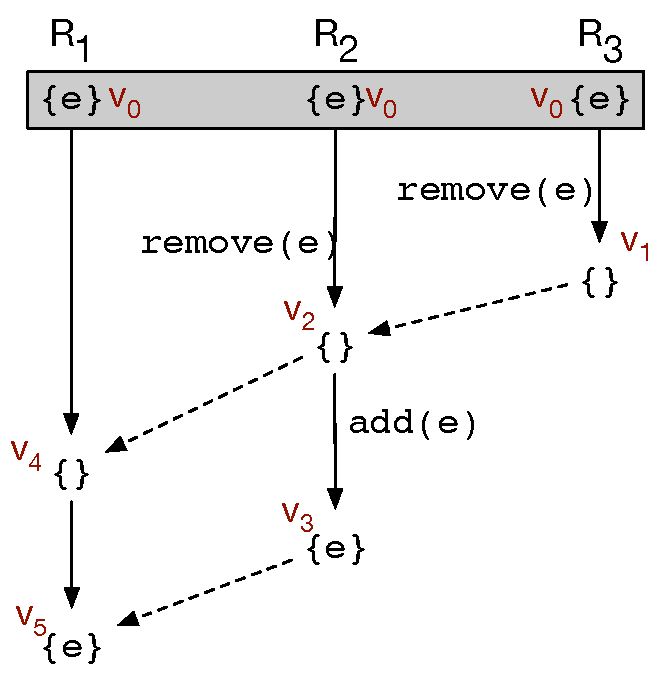
\includegraphics[scale=0.35]{Figures/mrdt-execs-1}
    \caption{}
    \label{fig:mrdt-execs-1}
  \end{subfigure}
  \begin{subfigure}[t]{0.44\columnwidth}
    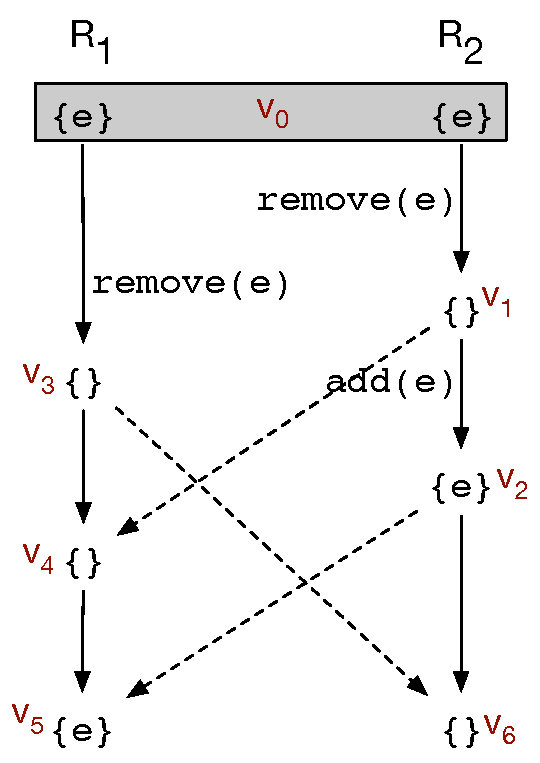
\includegraphics[scale=0.35]{Figures/mrdt-execs-2}
    \caption{}
    \label{fig:mrdt-execs-2}
  \end{subfigure}
\caption{Equivalent executions of Fig.~\ref{fig:crdt-execs} in
state-centric replication model. Dashed lines now denote state merges.}
\label{fig:mrdt-execs}
\end{figure}

\noindent\paragraph{A Mergeable Replicated Set} To demonstrate the
aforementioned intuitions we reconsider the executions from
Fig.~\ref{fig:crdt-execs}, this time in the state-centric replication
model. The cornerstone of the state-centric model is a three-way
\C{merge} function that merges concurrent versions of the state in
presence of their (lowest) common ancestor version. In our running
example, the state is a value of type \C{Set.t}, hence \C{Set.merge}
function would have the type signature:
\begin{center}
\C{Set.merge} : \C{Set.t} $\rightarrow$ \C{Set.t} $\rightarrow$ \C{Set.t}
$\rightarrow$ \C{Set.t}
\end{center}
The three arguments of \C{merge} correspond to the lowest common
ancestor (LCA) version and the two concurrent versions that
independently evolved from the LCA version. The LCA is a causal
ancestor of concurrent versions, hence causal consistency is built
into the replication model. The result of set merge, intuitively, must
contain the common elements in the two concurrent versions along with
any newly added elements in either versions. Concretely:
\begin{ocaml}
  let merge s(*lca*) s1 s2 = 
              (s1 $\cap$ s2) $\cup$ (s1 - s) $\cup$ (s2 - s)
\end{ocaml}
Equipped with the above set merge function, we can now consider the
equivalent execution of Fig.~\ref{fig:crdt-execs-1} in state-centric
model. The execution is shown in Fig.~\ref{fig:mrdt-execs-1}. The
initial version on all three replicas ($v_0$) is the singleton set
$\{e\}$. Applying operations to replicas creates new versions, e.g.,
$v_1$ on $R_3$. Changes can be propagated by merging versions, e.g.,
version $v_2$ on $R_2$ is a result of merging $v_0$ and $v_1$ in
presence of their lowest common ancestor (LCA) version
$v_0$\footnote{Versions $v_0$ and $v_1$ are not concurrent as the
  former is an ancestor of the latter. Merging $v_1$ into $v_0$ is
  nonetheless possible as $v_1$ is ahead of $v_0$ in causal order. In
  Git parlance this is a \emph{fast forward} merge.}.
Likewise $v_4$ on $R_1$ is created by merging $v_3$ and $v_0$ in
presence of their LCA $v_0$. By the end of the execution, versions
$v_4$ and $v_3$ at $R_1$ and $R_2$ (resp.) have witnessed the same set
of operations, hence are in agreement.\GK{fix this.}

\noindent\paragraph{Well-formed executions and the \quark runtime}
Convergence however is not an inherent virtue of the state-centric
replication model. Fig.~\ref{fig:mrdt-execs-2} shows the state-centric
analogue of the execution in Fig.~\ref{fig:crdt-execs-2} which
diverges. Here $R_1$ and $R_2$ start with version $v_0 \,=\, \{e\}$.
$R_2$ performs a \C{remove} and and an \C{add} making versions
$v_1$ and $v_2$ respectively. Simultaneously, $R_1$ performs a
\C{remove} to make $v_3$. Replica $R_1$ now obtains $R_2$'s changes by
merging versions $V_1$ and $v_2$ to make new versions $v_4$ and $v_5$
respectively. LCAs for these merges are $v_0$ and $v_1$. Concurrently,
$R_2$ obtains $R_1$'s changes by merging $v_3$ with $v_2$ (LCA =
$v_0$) to make $v_6$.  Now $R_1$ and $R_2$ have same set of changes
yet their final versions differ.

Note that the anamolous execution in Fig.~\ref{fig:mrdt-execs-2} could
have been avoided had the merges between $R_1$ and $R_2$ been
linearized. Fig.~\ref{fig:mrdt-execs-3} shows an execution that only
slightly differs from the one in Fig.~\ref{fig:mrdt-execs-2}. The
difference is that the merges in Fig.~\ref{fig:mrdt-execs-3} happen
linearly: first $R_1$ is merged into $R_2$ (bringing $R_1$'s
\C{remove}), then $R_2$ into $R_1$ (bringing $R_2$'s \C{remove}),
followed again by $R_2$ into $R_1$ (bringing $R_2$'s \C{add}). As a
result of such linearization, the final versions on $R_1$ and $R_2$
converge to the singleton set $\{e\}$. Note that there exist other
linearizations of merges; for instance, $R_1 \,\rightarrow\, R_2$
merge could be ordered between the two $R_2 \rightarrow R_1$ merges.
However, all linearizations result in the same final state $\{e\}$.
Another important point to note is that only the merges are
linearized; not the entire execution. In Fig.~\ref{fig:mrdt-execs-3},
both $R_1$ and $R_2$'s \C{remove}s remove the same element $e$, which
is not possible in a linearized execution. Leaving the execution
unconstrained is crucial to satisfy the limits imposed by the CAP
theorem on a highly-available partition-tolerant distributed system.

In the context of Fig.~\ref{fig:mrdt-execs-3}, it is quite clear what
linearization of merges means and how to enforce it via
synchronization (for e.g., wrapping each merge within a global lock).
In general however, the semantics of merge linearization isn't as cut
and dried. For instance, consider the execution in
Fig.~\ref{fig:mrdt-execs-4}. The four replicas involved in the
execution start with version $v_0 \,=\, \{e\}$. The replicas perform
local operations as shown in the figure to make versions $v_1$ to
$v_5$. Next they perform a series of merges to propagate local
changes. The merges can be ordered in time as following: first $R_2
\rightarrow R_1$, then $R_3 \rightarrow R_1$, then $R_2 \rightarrow
R_4$, and finally $R_3 \rightarrow R_4$. Despite linearly ordered in
time, the merges nonetheless result in divergent execution. The
problem here is that, although merges are executed linearly, the
execution graph does not reflect this linearity; merges of that end in
$R_1$ in Fig.~\ref{fig:mrdt-execs-4} are effectively concurrent with
those that end in $R_4$. This shows that simply synchronizing the
execution of merges does not necessarily result in convergence.

Our key insight to overcome this impasse is a \emph{well-formedness}
condition on execution graphs that ensures convergence of final
states. To understand well-formedness, let us contrast the bad
executions in Figs.~\ref{fig:mrdt-execs-2} and~\ref{fig:mrdt-execs-4}
against the good execution in Fig.~\ref{fig:mrdt-execs-3}. Observe
that in Fig.~\ref{fig:mrdt-execs-2}, \emph{every} pair of concurrent
versions on $R_1$ and $R_2$ have a unique lowest common ancestor
(LCA). For instance, LCA of $(v_5,v_6)$ is $v_6$, $(v_5,v_4)$ is
$v_3$, $(v_1,v_2)$ is $v_0$ and so on. By contrast in
Fig.~\ref{fig:mrdt-execs-2}, versions $v_5$ and $v_6$ have two LCAs,
namely $v_2$ and $v_3$. Both these versions are common ancestors of
$v_5$ and $v_6$, and both are \emph{lowest} in the sense that there do
not exist versions lower (in the execution graph) than $v_2$ and $v_3$
that are also common ancestors of $v_5$ and $v_6$. Likewise in
Fig.~\ref{fig:mrdt-execs-4}, versions $v_7$ and $v_9$ have two LCAs --
$v_2$ and $v_4$. Multiple LCAs is an indication that there exist
merges prior in the execution graph that are effectively concurrent.
Considering that our approach to convergence in state-centric model
crucially relies on linearity of merges, presence of multiple LCAs
opens up the possibility of divergence. We therefore define
well-formed execution graphs as those where LCAs for every pair of
concurrent versions is unique. As we prove in
Sec.~\ref{sec:formalization}, enforcing this structural
well-formedness condition indeed guarantees the convergence of
distributed executions. In Sec.~\ref{fig:implementation}, we describe
a distributed runtime called \quark whose primary purpose is to
enforce the well-formedness condition on distributed executions. The
runtime makes it possible to automatically promote ordinary data types
equipped with a merge function to convergent replicated data types.
Thus, extending the \C{Set} interface of Fig.~\ref{fig:ocaml-set} with
the two-line \C{Set.merge} function shown above is sufficient to
obtain a convergent replicated set data type.

The following section formalizes the aforementioned intuitions with
help of an abstract machine that generates only the well-formed
executions. \GK{fix this}


\section{Semantics of State-Centric Replication}
\label{sec:vc-semantics}

\begin{figure*}[t]
\begin{smathpar}
  \begin{array}{c}
    v\in\texttt{Versions/Vertices}\spc
    b\in\texttt{Branches}\spc
    c\in\texttt{CommitIds}\spc
    n\in\texttt{Values}\spc
    \cedge,\fedge,\medge \in \texttt{Edges}\spc
    G\in(\texttt{Vertices},\texttt{Edges})\\
    N : \texttt{Version} \rightarrow \texttt{Value}\spc
    C : \texttt{Version} \rightarrow \Pow{\texttt{CommitId}} \spc
    H : \texttt{Branch} \rightarrow \texttt{Version} \spc
    L : \texttt{Branch}\times\texttt{Branch} \rightarrow
    \texttt{Version}\\
  \end{array}
\end{smathpar}
%
\fbox {\( (G,N,C,H,L) \stepsto (G',N',C',H',L')\)} 
%
\bigskip

%
\begin{smathpar}
\begin{array}{c}
\RULE
{
  b\in dom(H)\spc
  v\not\in V\spc
  i\not\in codom(C)
}
{
  ((V,E),N,C,H,L) \stepsto (V \cup \{v\},\, E\cup\{H(b) \cedge v\},\,
  N[v \mapsto n],\,C[v \mapsto \{i\} \cup C(H(b))],\, H[b \mapsto v], L)
}
\spc
  [\rulelabel{Commit}]
\end{array}
\end{smathpar}
%

%
\begin{smathpar}
\begin{array}{c}
\RULE
{
  b\in dom(H)\spc
  b'\not\in dom(H) \spc
  v\not\in V\spc
}
{
  \hspace*{-0.3in}
  ((V,E),N,C,H,L) \stepsto (V \cup \{v\},\, E\cup\{H(b) \fedge v\},\,
  N[v \mapsto N(H(b))],\, C[v \mapsto C(H(b))],\\
  \hspace*{2in} 
  H[b' \mapsto v],\,
  L[(b',b) \mapsto H(b)]
                 [\{(b',b'') \mapsto L(b,b'') \,|\, b'' \neq b\}])
}
\spc
[\rulelabel{Fork}]
\end{array}
\end{smathpar}
%

%
\begin{smathpar}
\begin{array}{c}
\RULE
{
  b,b'\in dom(H)\spc
  C(H(b)) \supset C(L(b,b'))\spc
  C(H(b')) \supset C(L(b,b'))\\
% \neg(H(b') \reaches H(b))\spc
% \neg(H(b) \reaches H(b'))\\
  \forall (b''\in dom(H)).~L(b,b'') \reaches L(b',b'') 
    \disj L(b',b'') \reaches L(b,b'') \\
  n = {\sf merge}(N(L(b,b')),\, N(H(b)),\, N(H(b'))) \spc
  v \not\in V
}
{
  \hspace*{-1.5in}
  ((V,E),N,C,H,L) \stepsto (V \cup \{v\},\, E\cup\{H(b) \medge v, 
                                                 H(b') \medge v\},\\
    \hspace*{1in}
    N[v \mapsto n],\,
    C[v \mapsto C(H(b)) \cup C(H(b'))],\, H[b \mapsto v],\\
    \hspace*{1.8in}
    L[(b,b') \mapsto H(b') ]
     [\{(b,b'') \mapsto L(b',b'') \,|\, L(b,b'') \reaches L(b',b'')\}])
}
\spc
[\rulelabel{Merge}]
\end{array}
\end{smathpar}
%


%
\begin{smathpar}
\begin{array}{c}
\RULE
{
  b,b'\in dom(H)\spc
  C(H(b)) = C(L(b,b'))\spc
  C(H(b')) \supset C(L(b,b'))\\
% \neg(H(b') \reaches H(b))\spc
% H(b) \reaches H(b')\\
  \forall (b''\in dom(H)).~L(b,b'') \reaches L(b',b'') 
    \disj L(b',b'') \reaches L(b,b'') \spc
  v \not\in V
}
{
  \hspace*{-1.5in}
  ((V,E),N,C,H,L) \stepsto (V \cup \{v\},\, E\cup\{H(b) \medge v, 
                                                 H(b') \medge v\},\\
    \hspace*{1in}
    N[v \mapsto N(H(b'))],\,
    C[v \mapsto C(H(b'))],\,
    H[b \mapsto v],\\
    \hspace*{1.8in}
    L[(b,b') \mapsto H(b') ]
     [\{(b,b'') \mapsto L(b',b'') \,|\, L(b,b'') \reaches L(b',b'')\}])
}
\spc
[\rulelabel{FastFwd}]
\end{array}
\end{smathpar}
%

\caption{The semantics of \quark abstract machine inspired by the Git
version control system}
\label{fig:git-semantics}
\end{figure*}


In this section we present the formal semantics of our state-centric
replication scheme with linearized merges. As the informal development
from previous section suggests, our replication scheme is strongly
inspired by version control systems (VCS) such as Git~\cite{git}.  We
embrace this analogy in our formal development to manifest distributed
executions over replicated state with help of an abstract ``Git''
machine building a well-formed version history graph.  We show that
the version history graph thus generated has several desirable
properties including unique LCAs for every pair of versions, and
convergence of versions that include the same set of \emph{commits}.
We are however not concerned about the practical aspects of the system
yet; the subsequent sections gradually refine the abstract semantics
described here into a practical distributed system we call \quark. For
convenience, we refer to the abstract ``Git'' machine we describe here
also as \quark.

Fig.~\ref{fig:git-semantics} shows the operational semantics of the
\quark abstract machine. The machine admits the usual version control
operations, namely \rulelabel{Commit}, \rulelabel{Fork},
\rulelabel{Merge}, and \rulelabel{FastFwd}. Operation
\rulelabel{FastFwd} is a special case of merge which simply \emph{fast
forwards} a branch to a later version. A \emph{branch} is a linear
sequence of versions, which intuitively denotes the progressive
evolution of the state on a replica. The latest version of the branch,
called its \emph{head}, denotes the current state of the corresponding
replica. A new head version is created either by an
externally-initiated \emph{commit} (\rulelabel{Commit}) or by merging
the current head with a concurrent or causally-succeeding version from
a different branch (\rulelabel{Merge} and \rulelabel{FastFwd}
respectively). A new branch can be created by \emph{forking off} a
version on an existing branch (\rulelabel{Fork}). Although a version
control system admits more operations (e.g., ``rebase''), we observe
that these four basic actions are sufficient to capture the behavior
of an asynchronously replicated multi-versioned state machine.

The state of \quark abstract machine is a tuple $\Delta = (G,N,C,H,L)$, where:
\begin{itemize}
  \item $G = (V,E)$ is the version history DAG generated by the
    execution of the abstract machine. Vertices ($V$) of the graph are
    the set of all versions that ever existed during the execution.
    Edges ($E$) record the relationships between various versions. In
    particular, there are three kinds of edges corresponding to the
    three basic operations: commit ($\cedge$), merge ($\medge$), fork
    ($\fedge$). Fast forward, being a special case of merge, is also
    denoted by a merge edge ($\medge$). Existence of an edge $v_0
    \rightarrow  v_1$ denotes that versions $v_0$ and $v_1$ are related by
    some operation. For e.g., $v_0 \fedge v_1$ denotes that $v_1$ is a
    new version forked-off from the version $v_0$ using the
    \rulelabel{Fork} rule. As usual, \emph{path} relation is the
    reflexive transitive closure of the edge relation, i.e,
    $\reaches$.
%   \rulelabel{Fork}
%   rule (explained later) dictates that $v_0$ and $v_1$ are different
%   versions belonging to different branches, albeit denoting the 

  \item $N : \texttt{Version} \rightarrow \texttt{Value}$ is a
    (partial) function (i.e., a map) that mas versions to their
    values.  We distinguish versions from values as different versions
    on different branches may store the same value (e.g., the same
    string ``hello''), yet need to be uniquely identified. The domain
    of values is left uninterpreted except for the requirement that
    it be \emph{mergeable}, i.e., define a three-way \C{merge}
    function.

  \item $C : \texttt{Version} \rightarrow \Pow{\texttt{CommitId}}$
    maps a version $v$ to the set of commit ids included in that
    version. Each commit event during the execution is uniquely
    identified by a commit id (analogous to the Git's commit hash).
    The set of commit ids $C(v)$ therefore denotes the commit events
    that contributed to the version $v$. Intuitively, this represents
    the set of user-initiated operations that affected the value of
    this version.

  \item $H : \texttt{Branch} \rightarrow \texttt{Version}$ is an
    injective (partial) function that maps each branch to its head
    version. 

  \item $L: \texttt{Branch}\times\texttt{Branch} \rightarrow
    \texttt{Version}$ maps a pair of branches to the lowest common
    ancestor (LCA) version of their heads. We later prove the unique
    LCA property, so $L$ is indeed a (partial) function. Note that LCA
    of a pair of branches $b_1$ and $b_2$ need not necessarily lie on
    $b_1$ or $b_2$; it could also be a version on a different branch
    $b$. This happens, for e.g., if $b_1$ and $b_2$ alternatively
    merged the same version from $b$.
\end{itemize}

\paragraph{Notation} We let $v_{\odot}$ denote the initial version
(``root''), and $b_{\odot}$ denote the initial branch (``master'').
The execution of the abstract machine progresses by adding to the sets
$V$ and $E$, and updating the maps $N$, $C$, $H$, and $L$. We adopt
the usual update notation, e.g., $H[b \mapsto v]$ is a map $H'$ such
that $H'(b) = v$, and forall $b' \neq b$, $H'(b') = H(b')$.  Multiple
updates to a map are parsed left-associatively. Map $L$ is assumed to
be commutative, so $L[(b,b') \mapsto v]$ is equal to $L[(b,b') \mapsto
v][(b',b) \mapsto v]$; the former is used as a succinct replacement of
the latter. To update multiple bindings in $L$, we use the set
comprehension notation: given a branch $b$, $L[\{(b,b') \mapsto v
\,|\, \phi(b,b')\}]$ updates all bindings $(b,b')$ in $L$ to $v$,
where $b'$ is any branch such that $\phi(b,b')$ is true. Domain and
co-domain of a map $M$ is denoted $dom(M)$ and $codom(M)$
respectively.

\begin{definition}[Initial State and Version History Graph]
  The graph $G_{\odot} = (\{v_{\odot}\},\emptyset)$ is the initial
  version graph. The state $\Delta_{\odot}$ = $(G_{\odot},\,
  [v_{\odot} \mapsto b_{\odot}],\, [b_{\odot} \mapsto v_{\odot}],\,
  \emptyset)$ is the initial state.
\end{definition}

\noindent All executions of the abstract machine are assumed to start from the
initial state.

\begin{definition}[Ancestor]
  In version history DAG $G = (V,E)$, version $v_0 \in V$ is said
  to be a (causal) ancestor of $v_1 \in V$ iff $v_0 \reaches v_1$.
  Versions $v_0, v_1 \in V$ are causally related iff either $v_0
  \reaches v_1$ or $v_1 \reaches v_0$.
\end{definition}

% \begin{definition}[Common Ancestor] Common ancestor is defined for
%   versions and branches as following:
%   \begin{itemize} 
%     \item In $G = (V,E)$, a version $v\in V$ is called a common ancestor of
%       versions $v_1 \in V$ and $v_2 \in V$ iff $v \reaches v_1$ and $v \reaches
%       v_2$ in $G$.
%     \item In state $\Delta \,=\, ((V,E),N,C,H,L)$, $v\in V$ is called
%       a common ancestor of branches $b_1 \in dom(H)$ and $b_2 \in
%       dom(H)$ iff $v$ is a common ancestor of $H(b_1)$ and $H(b_2)$.
%   \end{itemize}
% \end{definition}

\begin{definition}[Lowest Common Ancestor (LCA)]
  In version history DAG $G = (V,E)$, a version $v\in$ is a lowest common
  ancestor of versions $v_1 \in V$ and $v_2 \in V$ iff:
  \begin{itemize}
    \item $v$ is a common ancestor of $v_1$ and $v_2$, i.e., $v
      \reaches v_1$ and $v \reaches v_2$, and
    \item There does not exist a $v'\in V$ such that $v'$ is a common
      ancestor of $v_1$ and $v_2$, and $v \reaches v'$.
  \end{itemize}
  LCA of a pair of branches is defined as the LCA of their heads.
\end{definition}

\paragraph{Rules} The rule \rulelabel{Commit}
(Fig.~\ref{fig:git-semantics}) describes committing a new version $v$
onto the branch $b$ updating its head. The value $n$ for the new
version is assumed to have been provided by whoever has invoked the
commit, e.g., the user. Intuitively, user invokes an RDT operation
(e.g., \C{add($e$)}) on the value of the current version to create the
new value $n$, and thus the new version $v$. A unique commit id $c$ is
assigned to this commit event and added to $C(v)$. The set $C(v)$
also contains all the commit ids from the previous version $H(b)$
since the new value $n$ is assumed to have been derived from the
previous value $N(H(b))$. The edge $H(b) \cedge v$ records this
dependency and also documents the progression of branch $b$. The LCA
map $L$ does not change as the only new edge is between the versions
of the same branch $b$.

\rulelabel{Fork} describes the semantics of forking a new branch $b'$
from the head of an existing branch $b$. The head of $b'$ is a new
version $v$ that shares the same commit set ($C(v)$) and value
($N(v)$) as its predecessor ($H(b)$). The lowest common ancestor (LCA)
of $b'$ and its parent $b$ is clearly the head of the parent $H(b)$ as
there does not exist a version $v$ lower than $H(b)$ that is an
ancestor of both $H(b)$ and $H(b')$. For every other branch $b''$,
$L(b',b'')$ is same as $L(b,b'')$. Fork operation could model, for
e.g., creating a new replica by forking off the current state of an
existing replica.

\rulelabel{Merge} describes the semantics of merging the head of a
branch $b'$ into $b$ resulting in an new version $v$ on $b$.
Intuitively, \rulelabel{Merge} models the information exchange between
replicas. The two pre-conditions specified using the strict superset
relation ($\supset$) require each of the merging versions, $H(b)$ and
$H(b')$, to include at least one commit not present in their common
ancestor $L(b,b')$. These conditions ensure that the merge is not
trivial (trivial merge is handled by \rulelabel{FastFwd}). The next
pre-condition is key to ensuring the uniqueness of LCAs and the
linearity of merges. It requires that, for every branch $b''$ in the
system, the LCA of $b''$ with merging branches $b$ and $b'$ be
causally related, i.e, $L(b,b'') \reaches L(b',b'') \disj L(b',b'')
\reaches L(b,b'')$. Fig.~\ref{fig:merge-precondition} helps visualize
this condition in the most general case when (\rom{1}). Branches $b$,
$b'$, and $b''$ are distinct, and (\rom{2}). Their LCAs $L(b,b'')$ and
$L(b',b'')$ lie on a distinct pair of branches not equal to $b$, $b'$,
and $b''$. In the figure, once you merge $b'$ into $b$, every version
$v$ that is an ancestor of $L(b',b'')$, i.e., $v \reaches L(b',b'')$,
will be  a common ancestor of $H(b)$ and $H(b'')$. Clearly,
$L(b',b'')$ is the lowest among such common ancestors. But the current
lowest common ancestor of $b$ and $b''$ is $L(b,b'')$. We therefore
end up with two lowest common ancestors -- $L(b',b'')$ and $L(b,b'')$,
\emph{unless} both are ancestrally related. Thus the pre-condition
$L(b,b'') \reaches L(b',b'') \disj L(b',b'') \reaches L(b,b'')$. If
$L(b',b'') \reaches L(b,b'')$, then $L(b,b'')$, the current LCA of $b$
and $b''$, is still the LCA after the merge. On the other hand, if
$L(b,b'') \reaches L(b',b'')$, then $L(b',b'')$ becomes the lowest
common ancestor of $b$ and $b''$ after the merge. Thus $L(b,b'')$
needs to be updated if and only if $L(b,b'') \reaches L(b',b'')$. The
conclusion of the \rulelabel{Merge} captures this update using the set
comprehension notation. It also updates the LCA of the merging
branches $L(b,b')$ to $H(b')$ since the head of $b'$ is merged into
$b$. Updates to the other components of the state (e.g., $C$) follow
the same rationale as previours rules. Two edges are added to $E$ as
the new version $v$ is a descendent of the two merging versions.

Another notable aspect of the \rulelabel{Merge} rule is the invocation
of the \C{merge} function on the values of the  merging versions and
their common ancestor to derive the result of the merge. As explained
above, our development is parameterized on the domain of values for
which a \C{merge} function is defined. No futher constraints are
imposed on \C{merge}. We use an uncurried version of \C{merge} to
avoid clutter.

\rulelabel{FastFwd} generalizes merge to the case when the merging
version $H(b')$ is a descendent of the version $H(b)$. In this case
$H'(b)$, the new head of $b$, needs to have the same value and same
set of commits as $H(b')$. Other premises and conclusions are similar
to the \rulelabel{Merge} rule. Note that we don't need a separate rule
for fast forward merge if \C{merge} satisfies the invariant that
$\forall n, n'.~ \C{merge}(n,n,n') \,=\, \C{merge}(n,n',n) \,=\, n$.
Having a separate rule lets us elide this constraint.

\paragraph{Properties} We now formalize the notable properties of the
abstract machine and its executions\footnote{
  The manaul proofs of the theorems and their Ivy
  formalization~\cite{ivy} can be found in the supplementary material.
}. 

\begin{lemma}[Uniqueness of LCA]
  \label{lem:lca-uniqueness}
  In every reachable state $\Delta = (G,N,C,H,L)$ of the abstract
  machine, every pair of branches $b_1, b_2 \in dom(H)$ has a unique
  LCA given by $L(b_1,b_2)$.
\end{lemma}

The intuition behind the proof is succinctly captured by
Fig.~\ref{fig:merge-precondition}, which is explained above.

\begin{lemma}[Commit sets grow monotonically]
  \label{lem:commit-monotonicity}
  In every reachable state $\Delta = ((V,E),N,C,H,L)$ of the abstract
  machine: Forall $v_1,v_2 \in V$, if $v_1 \reaches v_2$ then $C(v_1)
  \subseteq C(v_2)$.
\end{lemma}

Lemma~\ref{lem:commit-monotonicity} guarantees that merges never lose
a commit.

\begin{corollary}[Commit sets modulo LCA are disjoint]
  \label{lem:commit-disjointness}
  In every reachable state $\Delta = ((V,E),N,C,H,L)$ of the abstract
  machine: Forall distinct $b_1, b_2 \in dom(H)$, and $v_0, v_1, v_2
  \in V$ s.t.  $v_1 = H(b_1)$ and $v_2 = H(b_2)$ and $v_0 =
  L(b_1,b_2)$, the following is true: $(C(v_2) - C(v_0)) ~\cap~
  (C(v_1) - C(v_0)) = \emptyset$.
\end{corollary}

Corollary~\ref{lem:commit-disjointness} follows from
Lemmas~\ref{lem:lca-uniqueness} and~\ref{lem:commit-monotonicity}.

\begin{theorem}[{\bf Convergence}]
  \label{thm:convergence}
  In every reachable state $\Delta = ((V,E),N,C,H,L)$ of the abstract
  machine: Forall distinct $b_1, b_2 \in dom(H)$, and $v_1, v_2 \in V$
  such that $v_1 = H(b_1)$ and $v_2 = H(b_2)$, the following is true:
  $C(v_1) = C(v_2) \Rightarrow N(v_1) = N(v_2)$.
\end{theorem}

Theorem~\ref{thm:convergence} is the key result of this section. It
asserts that any two branches that witnessed the same set of commits
have the same value. Intuitively, this means that any two replicas
that witnessed the same set of user actions arrive at the same final
state \emph{regardless} of the order in which they are witnessed. 



\section{Concrete Semantics}
\label{sec:concrete-sem}

\begin{figure*}[t]
\begin{smathpar}
  \begin{array}{c}
    i,j\in\texttt{ReplicaIds}\spc
    b_i,b_j\in\texttt{Branches}\spc
    t\in\texttt{VersionVectors}\spc
    n\in\texttt{Values}\spc
%   \cedge,\fedge,\medge \in \texttt{Edges}\spc
%   G\in(\texttt{Vertices},\texttt{Edges})\\
    N : \texttt{VersionVector} \rightarrow \texttt{Value}\\
%   C : \texttt{Version} \rightarrow \Pow{\texttt{CommitId}} \spc
%   R : \texttt{ReplicaId} \rightarrow \texttt{Branch} \spc
    H : \texttt{ReplicaId} \rightarrow \texttt{Branch} \rightarrow \texttt{VersionVector} \spc
%   L : \texttt{Branch}\times\texttt{Branch} \rightarrow \texttt{Version}\\
    B : \texttt{ReplicaId} \rightarrow (\texttt{Branch} \times \mathbb{N}) \rightarrow \texttt{VersionVector} \spc
  \end{array}
\end{smathpar}
%
  \fbox {\( (B,N,H) \qstepsto (B',N',H')\)} 
%
%\bigskip

%
\begin{smathpar}
\begin{array}{c}
\RULE
{
  b_i\in dom(H_i)\spc
  t = H_i(b_i)\spc
  t' = t[b_i \mapsto t(b_i) + 1]\spc
}
{
  (B,N,H) \qstepsto (B_i[(b_i,t'(b_i)) \mapsto t'],\,
  N[t' \mapsto n],\, H_i[b_i \mapsto t'])
}
\spc
  [\rulelabel{Commit}]
\end{array}
\end{smathpar}
%

%
% \begin{smathpar}
% \begin{array}{c}
% \RULE
% {
%   b_i\in dom(H)\spc
%   b_j\not\in dom(H) \spc
%   t = H_i(b_i)\spc
%   t' = t[b_j \mapsto 1]
% }
% {
%   (B,N,H) \qstepsto (B_j[(b_j,1) \mapsto t'],\, N[t' \mapsto N(t)],\,
%         H_j[b_j \mapsto t'])
% }
% \spc
% [\rulelabel{Fork}]
% \end{array}
% \end{smathpar}
%

%
\begin{smathpar}
\begin{array}{c}
\RULE
{
  b_i,b_j\in dom(H_i)\spc
  \forall (k\in dom(H)).~b_k \in dom(H_i) \conj H_i(b_k) = H_k(b_k)\\
  t_i = H_i(b_i) \spc
  t_j = H_i(b_j)\spc
  t_l = t_i \sqcap t_j\spc
  t_l < t_i\spc
  t_l < t_j\spc
  t' = t_j \sqcup t_i[b_i \mapsto t_i(b_i)+1]\\
  \forall (k\in dom(H)).~
    (t_i \sqcap H_i(b_k)) \lesseqgtr (t_j \sqcap H_i(b_k))\spc
  n = {\sf merge}(N(t_l),\, N(H_i(b_i)),\, N(H_i(b_j))) 
}
{
  (B,N,H) \qstepsto (B_i[(b_i,t'(b_i)) \mapsto t'],
            N[t' \mapsto n],\, H_i[b_i \mapsto t'])
}
\spc
[\rulelabel{Merge}]
\end{array}
\end{smathpar}
%


%
% \begin{smathpar}
% \begin{array}{c}
% \RULE
% {
%   b_i,b_j\in dom(H_i)\spc
%   \forall (k\in dom(H)).~b_k \in dom(H_i) \conj H_i(b_k) = H_k(b_k)\\
%   t_i = H_i(b_i) \spc
%   t_j = H_i(b_j)\spc
%   t_i < t_j \spc
%   t' = t_j[b_i \mapsto t_i(b_i)+1]\spc
%   \forall (k\in dom(H)).~
%     (t_i \sqcap H_i(b_k)) \lesseqgtr (t_j \sqcap H_i(b_k))
%   %
% % \neg(H(b') \reaches H(b))\spc
% % H(b) \reaches H(b')\\
% }
% {
%   (B,N,H) \qstepsto (B_i[(b_i,t'(b_i)) \mapsto t'],
%             N[t' \mapsto N(t_j)],\, H_i[b_i \mapsto t'])
% }
% \spc
% [\rulelabel{FastFwd}]
% \end{array}
% \end{smathpar}
%



%
\begin{smathpar}
\begin{array}{c}
\RULE
{
  b_k\in dom(H_i)\spc
  b_k \in dom(H_j)\spc
  t = H_i(b_k) \spc
  t' = H_j(b_k)\spc
  t' > t
  %
% \neg(H(b') \reaches H(b))\spc
% H(b) \reaches H(b')\\
}
{
  (B,N,H) \qstepsto (B_i[(b_k,t(b_k)+n) \mapsto B_j(b_k,t(b_k)+n)
                          \,|\, n \in \{1,\ldots,t'(b_k) - t(b_k)\}],
            N,\, H_i[b_k \mapsto t'])
}
\spc
[\rulelabel{Sync}]
\end{array}
\end{smathpar}
%



\caption{The semantics of \quark distributed machine}
\label{fig:quark-semantics}
\end{figure*}


The \quark abstract machine of the previous section deliberately
ignores system-level concerns to focus on the semantics of
version-controlled state replication. In this section we present the
\quark \emph{distributed} machine that addresses the key system-level
concerns and provides a blueprint for a practical version-controlled
replicated state machine. We first reify the the one-to-one
correspondence between replicas and branches we assumed informally in
the previous section. This requires us to relax the assumption of the
state $\Delta$ being shared synchronously across all replicas. Next we
present an efficient method to track the version history with help
of vector clocks. Finally, we outline an algorithm for garbage
collecting older versions so that the version history need not grow
unboundedly.

Fig.~\ref{fig:quark-semantics} shows the operational semantics of the
distributed machine. The key difference from the abstract semantics of
Fig.~\ref{fig:git-semantics} is the presence of $\texttt{ReplicaId}$
indexing the components of the system state. We thus admit the
possibility of different replicas having different conceptions of the
state. Another major difference is the use of version
vectors~\cite{vectorclock} as identifiers and placeholders for
versions. A version vector of a version $v$ records the sequence
number of the last version from each branch that causally precedes $v$
(as per Def.~\ref{def:ancestor}).  Concretely, version vector is a map
from branches to natural numbers:
\begin{center}
  $\texttt{VersionVector}$ = $\texttt{Branch} \rightarrow \mathbb{N}$
\end{center}

The state of the distributed machine is the triple $\delta = (B,N,H)$.
Components $B$ and $H$ are indexed by $\texttt{ReplicaId}$ to let us
denote their replica-local copies. For instance, replica $i$'s copy of
the \emph{head map} $H$ is given by $H\;i$, which we abbreviate to
$H_i$ for notational convenience. Like $H$ in
Fig.~\ref{fig:git-semantics}, $H_i$ maps each branch to the version
vector of its head. Note that two replicas may be out of sync w.r.t
the information in $H$ and $B$.  For instance, $H_i(b)$ may not be
equal to $H_j(b)$ if replicas $i$ and $j$ are out of sync. On a
replica $i$, \emph{branch map} $B_i$ gives the version vector
corresponding to a particular sequence number on a branch. For
instance, the version vector of the first version on branch $b$ is
given by $B_i(b,1)$ on replica $i$. The value map $N$ maps version
vectors to their values. We assume a single copy of $N$ to simplify
the presentation. Generalizing Fig.~\ref{fig:quark-semantics} to allow
for replica-local copies of $N$ is straightforward.

Conspicuous by its absence in Fig.~\ref{fig:quark-semantics} is the
LCA map $L$, which we previously used to track the LCA version for
every pair of branches. The use of version vectors, coupled with the
unique LCA guarantee, obviates the need for an LCA map.  We can
instead identify the LCA of a pair of versions $v_1$ and $v_2$ by
computing the \emph{greatest lower bound} (GLB) of their version
vectors $t_1$ and $t_2$. Concretely:
\begin{center}
  $t_l \,=\, t_1 \sqcap t_2$
\end{center}
Where $t_l$ is the version vector of the LCA and $\sqcap$ is the GLB
operator. Conversely, the version vector identifying the result of a
merge can be computed as the \emph{least upper bound} (LUB) of the two
version vectors involved in the merge. Concretely:
\begin{center}
  $t_m \,=\, t_1 \sqcup t_2$
\end{center}
Where $t_1$ and $t_2$, and $t_m$ are the version vectors of the
merging versions and the result of the merge, respectively. For
technical reasons, however, we increment the component of $t_m$
corresponding to the current branch $b$ to signify that this is a new
version on $b$. So the actual version vector of the merge is $t_m' =
t_m[b \mapsto t_m(b)+1]$. The GLB and LUB operations on version
vectors are standard~\cite{vectorclock} -- GLB is computed by taking
the component-wise minimum, and LUB by taking their maximum. The
comparison of version vectors is also standard -- $t_1 < t_2$ iff
$\forall b.~t_1(b) < t_2(b)$. Clearly, not all version vectors are
comparable. We write $t_1 \lesseqgtr t_2$ if vectors $t_1$ and $t_2$
are comparable.

\paragraph{Notation and Conventions} We enforce a one-to-one mapping
between replicas and branches by adopting the convention that branch
$b_i$ always corresponds to replica $i$. Concretely this means that
replica $i$ only ever creates new versions on branch $b_i$. Also,
replica $i$ can only update its local copies of $H$ and $B$, i.e.,
$H_i$ and $B_i$. For e.g., $H_i[b_i \mapsto t]$ updates the head of
branch $b_i$ to $t$ on replica $i$.  Since $H_i$ is simply an
abbreviation of $H\;i$ in the formalism, $H_i[b_i \mapsto t]$ actually
expands to $H_i[i \mapsto b_i \mapsto t]$. We exploit this notation in
Fig.~\ref{fig:quark-semantics}. 
% When two replicas, $i$ and $j$, are involved in an update, e.g.,
% \rulelabel{Fork}, we write $H_{\tuplee{i,j}}[b_j \mapsto t]$ to mean
% $H[i \mapsto b_j \mapsto t][j \mapsto b_j \mapsto t]$.

\paragraph{Rules} The transition relation $\qstepsto$ of the \quark
distributed machine is defined in Fig.~\ref{fig:quark-semantics}.
Every transition rule of the abstract machine
(Fig.~\ref{fig:git-semantics}) has a corresponding rule for the
abstract machine. Fig.~\ref{fig:quark-semantics} however elides
\rulelabel{Fork} and \rulelabel{FastFwd} in the interest of space.
The rule \rulelabel{Commit} describes replica $i$ committing a new
version on the branch $b_i$ with the given value $n$.  The vector $t'$
for the new version is obtained from that of the previous version $t$
by incrementing the component $b_i$. The sequence number of the new
version on $b_i$ is $t'(b_i)$ and the branch map $B_i$ is updated to
reflect that. Note that for all $j \neq i$, $H_j$ and $B_j$ remain
unchanged indicating that other replicas are not (yet) aware of this
commit.
%
\rulelabel{Fork} forks off a new branch $b_j$ from $b_i$. A new
replica $j$ is assumed to take over $b_j$. The version vector $t'$ of
the branch head now has a new component $b_j$ mapped to $1$ to denote
this is the first version on $b_j$. Map $B_j$ is updated accordingly.
Value $N(t')$ is same as its parent $N(t)$.

\rulelabel{Merge} describes the semantics of replica $i$ merging a
concurrent version from a (remote) replica $j$. The merging versions
are heads of their respective branches $b_i$ and $b_j$.  Like its
counterpart in Fig.~\ref{fig:git-semantics}, \rulelabel{Merge} insists
that the LCAs of every other branch $b_k$ with $b_i$ and $b_j$ be
causally related. This condition is however expressed in terms of
version vectors with help of the GLB ($\sqcap$) and comparison
($\lesseqgtr$) operators. For the LCA determination to be sound,
the merging replica $i$ needs to have an accurate conception of the
current version history. Furthermore, there cannot be a concurrent
merge happening elsewhere that undermines the judgment of replica $i$
(reg. the safety of $i \leftarrow j$ merge). These requirements are
enforced by the premise $\forall (k\in dom(H)).~b_k \in dom(H_i) \conj
H_i(b_k) = H_k(b_k)$, which insists that replica $i$'s knowledge of
every other branch $k$ be current. This condition effectively
linearizes merges by requiring a merge to either \emph{see} or
\emph{be seen} by every other merge. In practice this is achieved
through global coordination (Sec.~\ref{sec:implementation}). Note that
\rulelabel{Merge} only preempts a concurrent \rulelabel{Merge}, not a
concurrent \rulelabel{Commit}. A remote replica $k$ is allowed to keep
committing new versions on to $b_k$ even as it remains unaware of the
merge on replica $i$. Such leniency is imperative if the system were
to retain the performance benefits of asynchronous replication.
% \rulelabel{FastFwd} is similar to \rulelabel{Merge}, so we don't
% discuss it separately.

The rule \rulelabel{Sync} captures asynchronous communication between
a pair of replicas ($i$ and $j$) to get one of them ($i$) up-to-date
with the other ($j$).  Unlike the other rules, \rulelabel{Sync} does
not extend the version history graph, and therefore has no counterpart
in Fig.~\ref{fig:git-semantics}. It merely updates replica $i$'s
knowledge of branch $b_k$ if replica $j$ happens to have later updates
from $k$, i.e., $H_j(b_k)$ happens to be ahead of $H_i(b_k)$. The new
versions on $b_k$ known to $j$ but not $i$ are then simply replicated
at $i$.

\paragraph{Properties} The Unique LCA
(Lemma~\ref{lem:lca-uniqueness}), Convergence
(Theorem~\ref{thm:convergence}, and Progress
(Theorem~\ref{thm:progress}) properties have been re-defined for the
\quark distributed machine and automatically proven correct in
Ivy~\cite{ivy}. 

\paragraph{Garbage Collection} One downside of the distributed
semantics in Fig.~\ref{fig:quark-semantics} is that maps $B$ and $N$
that together track the version history grow monotonically as the
execution progresses and new versions are created. Fortunately, this
is easy to address as the execution only needs finite version history
to compute LCAs. Since LCA version vectors monotonically increase,
older versions with vectors less than the least known LCA vector can
simply be garbage-collected. Moreover, a replica can make this
decision locally without having to synchronize with its peers. In
practice, applications may prefer to flush out older version history
to a stable storage from where it can be re-created as necessary.



%% Acknowledgments
\begin{acks}                            %% acks environment is optional
                                        %% contents suppressed with 'anonymous'
  %% Commands \grantsponsor{<sponsorID>}{<name>}{<url>} and
  %% \grantnum[<url>]{<sponsorID>}{<number>} should be used to
  %% acknowledge financial support and will be used by metadata
  %% extraction tools.
  This material is based upon work supported by the
  \grantsponsor{GS100000001}{National Science
    Foundation}{http://dx.doi.org/10.13039/100000001} under Grant
  No.~\grantnum{GS100000001}{nnnnnnn} and Grant
  No.~\grantnum{GS100000001}{mmmmmmm}.  Any opinions, findings, and
  conclusions or recommendations expressed in this material are those
  of the author and do not necessarily reflect the views of the
  National Science Foundation.
\end{acks}


%% Bibliography
%\bibliography{bibfile}


%% Appendix
\appendix
\section{Appendix}

Text of appendix \ldots

\end{document}
